\section{交换积分}

\begin{quotation}
``我们一直被狄拉克的想法的不可理解的神奇所烦恼。
为了避开这些烦恼,我现在不想这些问题了,
转而去想一想磁铁的问题,于是做出来了这件工作。''\qquad 海森堡
\end{quotation}

\subsection{交换积分}

现在考虑两个电子, 我们既考虑轨道运动$\psi(\vec r)$,
也考虑自旋的运动$\chi (s_z)$, 总波函数$\Psi$, 我们写成相乘的形式,
其实就是直接乘积$\{\psi\} \otimes \{\chi\}$的形式:


\begin{equation*}
    \Psi(\vec r_1, \vec r_2; s_{1z}, s_{2z}) = \psi(\vec r_1, \vec r_2) \chi(s_{1z}, s_{2z})
\end{equation*}


由于电子是费米子, $\Psi$应该是反对称的, 分两种情况:

\begin{eqnarray*}
% \nonumber to remove numbering (before each equation)
  \Psi_A &=& \psi_S \cdot \chi_A \\
  \Psi_A &=& \psi_A \cdot \chi_S
\end{eqnarray*}

即: 如轨道部分是对称的$\psi_S$, 自旋部分就是反对称的$\chi_A$,
自旋单态; 如轨道部分是反对称的$\psi_A$, 自旋部分就是对称的$\chi_S$,
自旋三重态。

考虑两电子系统, 单电子哈密顿量是$\hat h$, 能量本征值是$\{E_n\}$,
对应的本征态是$\{\phi_n\}$, 即:

\begin{eqnarray*}
% \nonumber to remove numbering (before each equation)
  \hat h(\vec r_1) \phi_n(\vec r_1) &=& E_n \phi_n(\vec r_1) \\
  \hat h(\vec r_2) \phi_n(\vec r_2) &=& E_n \phi_n(\vec r_2)
\end{eqnarray*}

若不考虑电子和电子之间的相互作用$\hat H'(|\vec r_1 - \vec r_2|)$,
则哈密顿量为:

\begin{equation*}
    \hat H_0 = \hat h_1 + \hat h_2
\end{equation*}

若考虑$\hat H'$, 总哈密顿量为:

\begin{equation*}
    \hat H = \hat H_0 + \hat H'_{1,2}
\end{equation*}

我们的思路是先考虑$\hat H_0$, 然后再考虑$\hat H'$, 把$\hat
H'$当作微扰来考虑.

(1)先考虑基态, 基态两个电子都处在各自``单电子的基态''上, $E_0 =
2E_1$, $\psi_S= \phi_1(\vec r_1)\phi_1(\vec r_2)$, $\chi_A = \left|
\text{spin singlet} \right\rangle$
电子电子间的相互作用体现为能量的修正:

\begin{equation*}
    \Delta E = \left\langle {\vec r_1, \vec r_2; s_{1z}, s_{2z}} \left| \hat H'(|\vec r_1 - \vec r_2|) \right| {\vec r_1, \vec r_2; s_{1z}, s_{2z}} \right\rangle
\end{equation*}

由于轨道自由度和自旋自由度是分开的,
所以我们对轨道部分和自旋部分分别求量子力学平均。

\begin{equation*}
\Delta E = \left\langle {\psi_S( \vec r_1, \vec r_2)} \left| \hat
H'(|\vec r_1 - \vec r_2|) \right| {\psi_S(\vec r_1, \vec r_2)}
\right\rangle \cdot \left\langle \chi_A(s_{1z},s_{2z}) |
\chi_A(s_{1z},s_{2z}) \right\rangle
\end{equation*}

这里:$\left\langle \chi_A(s_{1z},s_{2z}) | \chi_A(s_{1z},s_{2z})
\right\rangle =1 $, (归一性)

那么:

\begin{eqnarray*}
% \nonumber to remove numbering (before each equation)
  \Delta E &=& \left\langle {\psi_S( \vec r_1, \vec r_2)} \left| \hat
H'(|\vec r_1 - \vec r_2|) \right| {\psi_S(\vec r_1, \vec r_2)}
\right\rangle \\
  {} &=& \int \phi_1^*(\vec r_1) \phi_1^*(\vec r_2) \hat H'(|\vec r_1 - \vec
  r_2|) \phi_1(\vec r_1) \phi_1(\vec r_2) d \vec r_1 \vec r_2 \\
  {} &=& \int |\phi_1(\vec r_1)|^2 H'(|\vec r_1 - \vec
  r_2|) |\phi_1(\vec r_2)|^2 d \vec r_1 \vec r_2 \\
  {} &=& \int \rho_1(\vec r_1) H'(|\vec r_1 - \vec r_2|) \rho_2(\vec r_2) d \vec r_1 \vec r_2
\end{eqnarray*}

这个式子有直观的物理含义, 即考虑``电子---电子''相互作用后,
电子1和电子2间按几率密度``积分''得到的静电势能之和。

(2)现在考虑第一激发态, 即1个电子在1态, 另一个电子在2态,
则这两个电子既可以处在自旋单态, 也可以处在自旋三重态。

如果处在自旋单态$\chi_A$:


\begin{equation*}
    \Psi_A  = \frac{1}{\sqrt 2}\left(\psi_1(r_1)\psi_2(r_2)+
    \psi_2(r_1)\psi_1(r_2)\right) \frac{1}{\sqrt 2} \left( \chi_+\chi_- - \chi_-\chi_+ \right)
\end{equation*}

计算对能量的微扰$\Delta E$,

\begin{center}
$\Delta E = \frac{1}{2} \int \left( \psi_1^*(r_1)\psi_2^*(r_2)+
\psi_2^*(r_1)\psi_1^*(r_2) \right) H' \times \left(
\psi_1(r_1)\psi_2(r_2)+ \psi_2(r_1)\psi_1(r_2) \right) d r_1 d r_2$
\end{center}

共四项:

\begin{eqnarray*}
{} & {} & \frac{1}{2}\int |\psi_1(r_1)|^2H'|\psi_2(r_2)|^2dr_1dr_2 \\
{} & {} & \frac{1}{2}\int |\psi_2(r_1)|^2H'|\psi_1(r_2)|^2dr_1dr_2 \\
{} & {} & \frac{1}{2}\int \psi_1^*(r_1)\psi_2(r_1) H'\psi_2^*(r_2)\psi_1(r_2)
dr_1dr_2 \\
{} & {} & \frac{1}{2}\int \psi_2^*(r_1)\psi_1(r_1) H'\psi_1^*(r_2)\psi_2(r_2)
dr_1dr_2
\end{eqnarray*}

如果处在自旋三重态$\chi_S$:

\begin{equation*}
\Psi_A = \frac{1}{\sqrt 2}\left(\psi_1(r_1)\psi_2(r_2) -
\psi_2(r_1)\psi_1(r_2)\right) \chi_S
\end{equation*}

那么:

\begin{center}
$\Delta E = \frac{1}{2} \int \left( \psi_1^*(r_1)\psi_2^*(r_2)-
\psi_2^*(r_1)\psi_1^*(r_2) \right) H' \times \left(
\psi_1(r_1)\psi_2(r_2)- \psi_2(r_1)\psi_1(r_2) \right) d r_1 d r_2$
\end{center}


共四项:

\begin{eqnarray*}
{}&{}& \frac{1}{2}\int |\psi_1(r_1)|^2H'|\psi_2(r_2)|^2dr_1dr_2\\
{}&{}&\frac{1}{2}\int |\psi_2(r_1)|^2H'|\psi_1(r_2)|^2dr_1dr_2\\
{}&{}&-\frac{1}{2}\int \psi_1^*(r_1)\psi_2(r_1) H'\psi_2^*(r_2)\psi_1(r_2) dr_1dr_2 \\
{}&{}&-\frac{1}{2}\int \psi_2^*(r_1)\psi_1(r_1) H'\psi_1^*(r_2)\psi_2(r_2) dr_1dr_2
\end{eqnarray*}

如果我们定义直接积分(K)为:

\begin{equation*}
K = \int |\psi_1(r_1)|^2H'|\psi_2(r_2)|^2dr_1dr_2
\end{equation*}

交换积分(J,也叫交换能)为:

\begin{equation*}
J = \int \psi_1^*(r_1)\psi_2(r_1) H'\psi_2^*(r_2)\psi_1(r_2)
dr_1dr_2
\end{equation*}

那么:

\begin{eqnarray*}
% \nonumber to remove numbering (before each equation)
  \Delta E(\text{spin singlet}) &=& K+J \\
  \Delta E(\text{spin triplet}) &=& K-J
\end{eqnarray*}


这两个能量哪一个更低呢?对He原子而言, 交换积分$J > 0$,
${}^3S_1$态(正氦)的能量($ K - J $)低于${}^1S_0$态(仲氦)的能量($ K + J$),
但基态是${}^1S_0$(仲氦)的态。

\index{Exchange interaction: 交换作用}

三重态与单态之间没有跃迁,所以它们各自内部的跃迁产生了两套相互独立的光谱。单态能级间的跃迁产生简单的单线光谱,而三重态能级间的跃迁产生的光谱有复杂的结构。由于氦出现了两套光谱,所以早期人们曾设想存在两种氦,这就是正氦和仲氦名称的由来。

\subsection{海森堡模型}

\begin{figure}[h]
\begin{center}
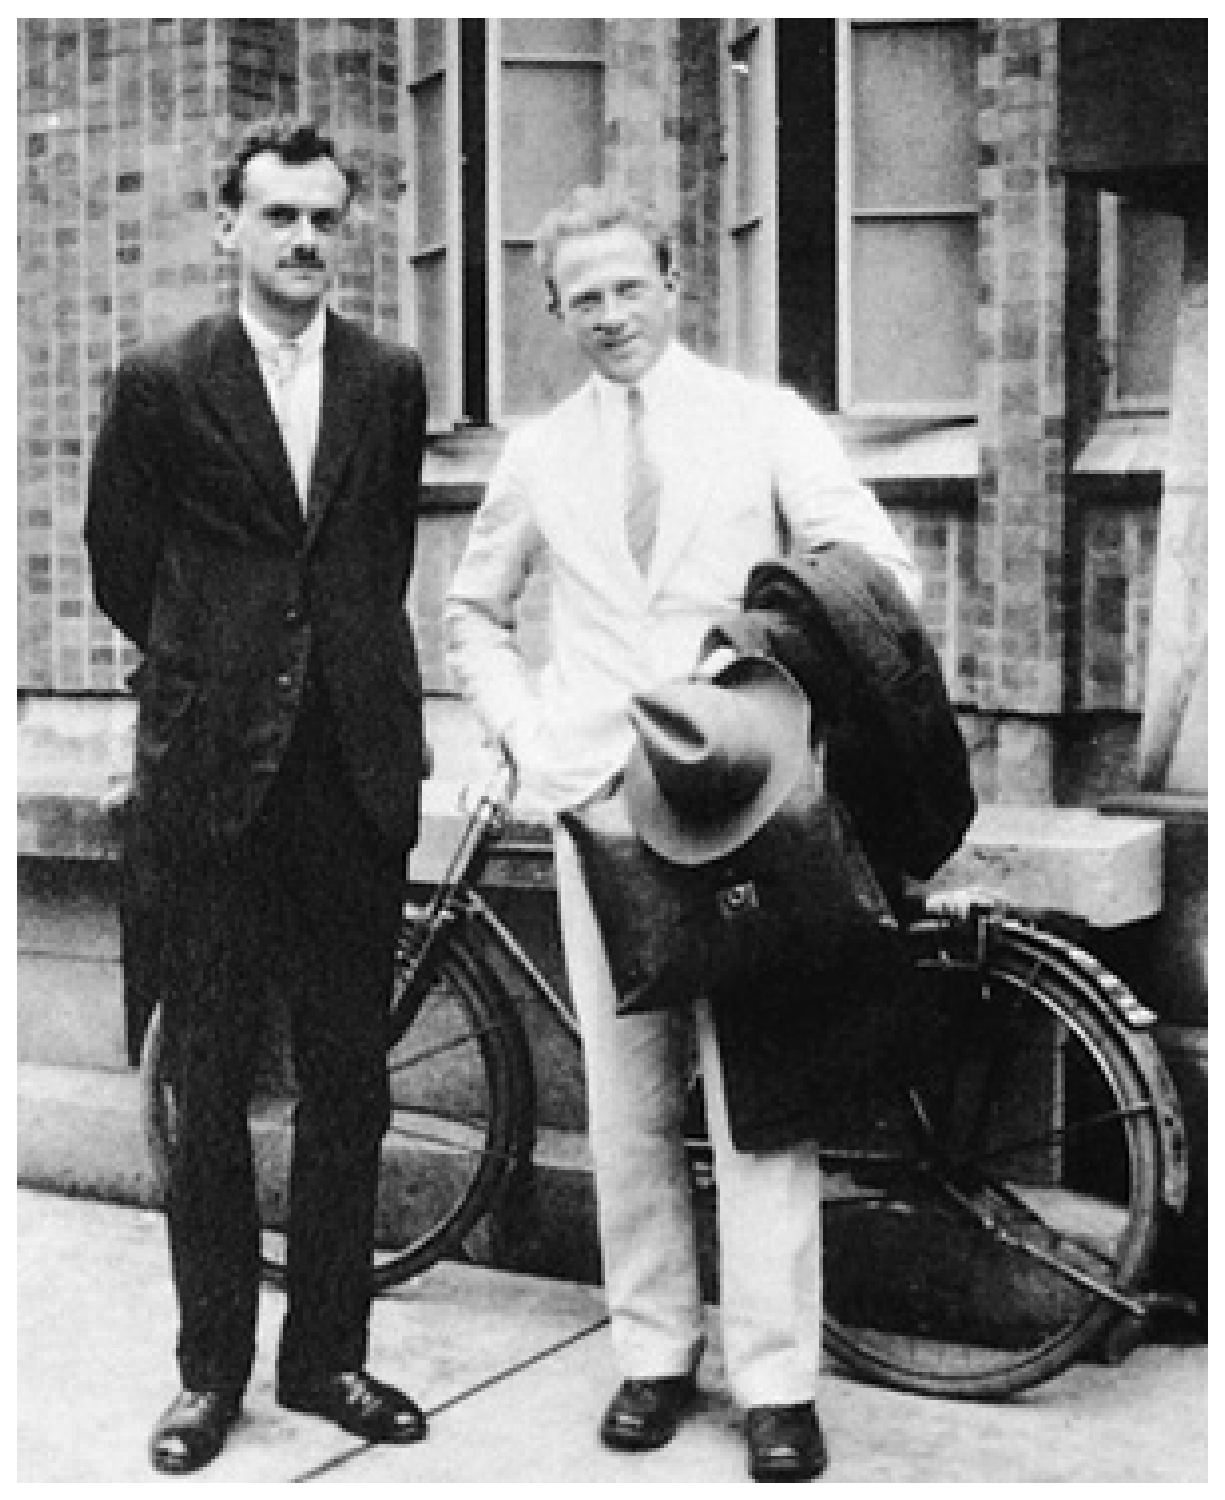
\includegraphics[clip,width=6cm]{IdenticalParticles/heisenberg-dirac.ps}
\caption{海森堡与狄拉克}
\end{center}
\end{figure}

海森堡利用交换能概念,解释了磁性的来源,并提出了海森堡模型。

考虑双原子分子:氢分子\footnote{参考周士勋《量子力学教程》第236页},忽略原子核的运动、自旋轨道相互作用、自旋之间相互作用:

\begin{equation}\label{32-3-1}
H = - \frac{\hbar^2}{2m}\left(\nabla_1^2 + \nabla_2^2 \right) + \frac{e^2}{4 \pi \varepsilon_0} \left( - \frac{1}{r_{1A}} - \frac{1}{r_{2B}} - \frac{1}{r_{1B}} - \frac{1}{r_{2A}} +  \frac{1}{r_{12}} +  \frac{1}{r_{AB}} \right)
\end{equation}


把$H' = \frac{{e^2 }}{{4\pi \varepsilon _0 }}\left( { - \frac{1}{{\left| {\mathord{\buildrel{\lower3pt\hbox{$\scriptscriptstyle\rightharpoonup$}}
\over r} _1  - \mathord{\buildrel{\lower3pt\hbox{$\scriptscriptstyle\rightharpoonup$}}
\over r} _B } \right|}} - \frac{1}{{\left| {\mathord{\buildrel{\lower3pt\hbox{$\scriptscriptstyle\rightharpoonup$}}
\over r} _2  - \mathord{\buildrel{\lower3pt\hbox{$\scriptscriptstyle\rightharpoonup$}}
\over r} _A } \right|}} + \frac{1}{{\left| {\mathord{\buildrel{\lower3pt\hbox{$\scriptscriptstyle\rightharpoonup$}}
\over r} _1  - \mathord{\buildrel{\lower3pt\hbox{$\scriptscriptstyle\rightharpoonup$}}
\over r} _2 } \right|}} + \frac{1}{{\left| {\mathord{\buildrel{\lower3pt\hbox{$\scriptscriptstyle\rightharpoonup$}}
\over r} _A  - \mathord{\buildrel{\lower3pt\hbox{$\scriptscriptstyle\rightharpoonup$}}
\over r} _B } \right|}}} \right)$当作微扰处理。


对于自旋三重态(自旋平行):$E^S  = 2E_H  + \frac{{e^2 }}{{4\pi \varepsilon _0 \left| {\mathord{\buildrel{\lower3pt\hbox{$\scriptscriptstyle\rightharpoonup$}}
\over r} _A  - \mathord{\buildrel{\lower3pt\hbox{$\scriptscriptstyle\rightharpoonup$}}
\over r} _B } \right|}} + \frac{{K - J}}{{1 - \Delta ^2 }}$

对于自旋单态(自旋反平行):$E^A  = 2E_H  + \frac{{e^2 }}{{4\pi \varepsilon _0 \left| {\mathord{\buildrel{\lower3pt\hbox{$\scriptscriptstyle\rightharpoonup$}}
\over r} _A  - \mathord{\buildrel{\lower3pt\hbox{$\scriptscriptstyle\rightharpoonup$}}
\over r} _B } \right|}} + \frac{{K + J}}{{1 + \Delta ^2 }}$

其中:

$\Delta  = \int {d\mathord{\buildrel{\lower3pt\hbox{$\scriptscriptstyle\rightharpoonup$}}
\over r} _1 \psi \left( {\mathord{\buildrel{\lower3pt\hbox{$\scriptscriptstyle\rightharpoonup$}}
\over r} _1  - \mathord{\buildrel{\lower3pt\hbox{$\scriptscriptstyle\rightharpoonup$}}
\over r} _A } \right)\psi \left( {\mathord{\buildrel{\lower3pt\hbox{$\scriptscriptstyle\rightharpoonup$}}
\over r} _1  - \mathord{\buildrel{\lower3pt\hbox{$\scriptscriptstyle\rightharpoonup$}}
\over r} _B } \right)} $

$\begin{array}{l}
K = \frac{{e^2 }}{{4\pi \varepsilon _0 }}\int d\mathord{\buildrel{\lower3pt\hbox{$\scriptscriptstyle\rightharpoonup$}}
\over r} _1 d\mathord{\buildrel{\lower3pt\hbox{$\scriptscriptstyle\rightharpoonup$}}
\over r} _2 \left| {\psi \left( {\mathord{\buildrel{\lower3pt\hbox{$\scriptscriptstyle\rightharpoonup$}}
\over r} _1  - \mathord{\buildrel{\lower3pt\hbox{$\scriptscriptstyle\rightharpoonup$}}
\over r} _A } \right)} \right|^2 \left| {\psi \left( {\mathord{\buildrel{\lower3pt\hbox{$\scriptscriptstyle\rightharpoonup$}}
\over r} _2  - \mathord{\buildrel{\lower3pt\hbox{$\scriptscriptstyle\rightharpoonup$}}
\over r} _B } \right)} \right|^2  \\ \times  \left( {\frac{1}{{\left| {\mathord{\buildrel{\lower3pt\hbox{$\scriptscriptstyle\rightharpoonup$}}
\over r} _1  - \mathord{\buildrel{\lower3pt\hbox{$\scriptscriptstyle\rightharpoonup$}}
\over r} _2 } \right|}} - \frac{1}{{\left| {\mathord{\buildrel{\lower3pt\hbox{$\scriptscriptstyle\rightharpoonup$}}
\over r} _2  - \mathord{\buildrel{\lower3pt\hbox{$\scriptscriptstyle\rightharpoonup$}}
\over r} _A } \right|}} - \frac{1}{{\left| {\mathord{\buildrel{\lower3pt\hbox{$\scriptscriptstyle\rightharpoonup$}}
\over r} _1  - \mathord{\buildrel{\lower3pt\hbox{$\scriptscriptstyle\rightharpoonup$}}
\over r} _B } \right|}}} \right) \\
\end{array}$

$\begin{array}{l}
 J = \frac{{e^2 }}{{4\pi \varepsilon _0 }}\int {d\mathord{\buildrel{\lower3pt\hbox{$\scriptscriptstyle\rightharpoonup$}}
\over r} _1 d\mathord{\buildrel{\lower3pt\hbox{$\scriptscriptstyle\rightharpoonup$}}
\over r} _2 \psi ^* \left( {\mathord{\buildrel{\lower3pt\hbox{$\scriptscriptstyle\rightharpoonup$}}
\over r} _1  - \mathord{\buildrel{\lower3pt\hbox{$\scriptscriptstyle\rightharpoonup$}}
\over r} _A } \right)\psi ^* \left( {\mathord{\buildrel{\lower3pt\hbox{$\scriptscriptstyle\rightharpoonup$}}
\over r} _2  - \mathord{\buildrel{\lower3pt\hbox{$\scriptscriptstyle\rightharpoonup$}}
\over r} _B } \right)\psi \left( {\mathord{\buildrel{\lower3pt\hbox{$\scriptscriptstyle\rightharpoonup$}}
\over r} _1  - \mathord{\buildrel{\lower3pt\hbox{$\scriptscriptstyle\rightharpoonup$}}
\over r} _B } \right)\psi \left( {\mathord{\buildrel{\lower3pt\hbox{$\scriptscriptstyle\rightharpoonup$}}
\over r} _2  - \mathord{\buildrel{\lower3pt\hbox{$\scriptscriptstyle\rightharpoonup$}}
\over r} _A } \right)}  \\
  \times \left( {\frac{1}{{\left| {\mathord{\buildrel{\lower3pt\hbox{$\scriptscriptstyle\rightharpoonup$}}
\over r} _1  - \mathord{\buildrel{\lower3pt\hbox{$\scriptscriptstyle\rightharpoonup$}}
\over r} _2 } \right|}} - \frac{1}{{\left| {\mathord{\buildrel{\lower3pt\hbox{$\scriptscriptstyle\rightharpoonup$}}
\over r} _2  - \mathord{\buildrel{\lower3pt\hbox{$\scriptscriptstyle\rightharpoonup$}}
\over r} _A } \right|}} - \frac{1}{{\left| {\mathord{\buildrel{\lower3pt\hbox{$\scriptscriptstyle\rightharpoonup$}}
\over r} _1  - \mathord{\buildrel{\lower3pt\hbox{$\scriptscriptstyle\rightharpoonup$}}
\over r} _B } \right|}}} \right) \\
 \end{array}$

如果交换积分$J>0$,自旋三重态为能量的基态,对应为自旋平行;
如果交换积分$J<0$,自旋单态为能量基态,对应为自旋反平行。

\begin{eqnarray*}
\widehat S_1  \cdot \widehat S_2 \chi ^S \left( {s_{1z} ,s_{2z} } \right) & = & \frac{1}{2}\left( {S^2  - S_1^2  - S_2^2 } \right)\chi ^S \left( {s_{1z} ,s_{2z} } \right) \\
{} & = & \frac{1}{2}\left( {2\hbar ^2  - \frac{3}{2}\hbar ^2 } \right)\chi ^S \left( {s_{1z} ,s_{2z} } \right) = \frac{{\hbar ^2 }}{4}\chi ^S \left( {s_{1z} ,s_{2z} } \right)
\end{eqnarray*}

\begin{eqnarray*}
\widehat S_1  \cdot \widehat S_2 \chi ^A \left( {s_{1z} ,s_{2z} } \right) & = & \frac{1}{2}\left( {S^2  - S_1^2  - S_2^2 } \right)\chi ^A \left( {s_{1z} ,s_{2z} } \right) \\
{} & = & \frac{1}{2}\left( {0\hbar ^2  - \frac{3}{2}\hbar ^2 } \right)\chi ^A \left( {s_{1z} ,s_{2z} } \right) =  - \frac{{3\hbar ^2 }}{4}\chi ^A \left( {s_{1z} ,s_{2z} } \right)
\end{eqnarray*}

能量修正:$\Delta E \propto  - JS_1  \cdot S_2 $

把交换作用推广到晶格系统,哈密顿可写为:

\begin{equation}\label{heisenberg model}
H =  - \sum\limits_{i,j} {J_{ij} \vec S_i  \cdot \vec S_j }
\end{equation}


\index{Heisenberg model: 海森堡模型}


这就是著名的海森堡模型, $J_{ij} $表示不同格点间的交换积分。如果$J>0$,基态是铁磁(FM)的;如果$J<0$,基态是反铁磁(AFM)的。

不同格点自旋的点积$S_i  \cdot S_j $,如果我们只考虑z方向的贡献:

\begin{equation}\label{ising model}
H_z  =  - \sum\limits_{i,j} {J_{ij} S_i^z  \cdot S_j^z }
\end{equation}

就得到伊辛模型(Ising Model)。

\index{Ising model: 伊辛模型}


如我们只考虑x-y方向的贡献:

\begin{equation}\label{xy model}
H_{xy}  =  - \sum\limits_{i,j} {J_{ij} \left( {S_i^x  \cdot S_j^x  + S_i^y  \cdot S_j^y } \right)}
\end{equation}

就得到XY模型(XY Model)。

\index{XY model: XY模型}

海森堡模型、伊辛模型以及XY模型在磁性理论、高温超导理论、膜生物物理等领域有广泛的应用。

\subsection{两自旋问题}

\subsubsection{两个自旋$1/2$耦合}

哈密顿量为:

\begin{equation}\label{two-spin-half}
  H = J S_1 \cdot S_2
\end{equation}

为了计算的简便把哈密顿量用升降算符($S^{\pm}$)和第三分量($S_z$)表示:

\begin{equation}\label{use-raising-lowering-operators}
J S_1 \cdot S_2 = \frac{J}{2} (S_1^+ S_2^- + S_1^-S_2^+) + J S_1^z
S_2^z
\end{equation}


这里:$S^+ = S_x + i S_y = \frac{\hbar}{2} (\sigma_x + i \sigma_y) =
\hbar \left( {\begin{array}{*{20}c}
   0 & 1  \\
   0 & 0  \\
\end{array}} \right)$
,$S^- = \hbar \left( {\begin{array}{*{20}c}
   0 & 0  \\
   1 & 0  \\
\end{array}} \right)$, 满足:


\begin{equation}\label{raising-lowering-property}
 S^+ \downarrow = \hbar \uparrow , S^- \uparrow = \hbar \downarrow
\end{equation}


取直接乘积表示:$\left| 1 \right\rangle = \uparrow \uparrow$
;$\left| 2 \right\rangle = \uparrow \downarrow$ ;$\left| 3
\right\rangle = \downarrow \uparrow$ ;$\left| 4 \right\rangle =
\downarrow \downarrow$

这里假设我们可以对自旋进行编号, 左边的箭头表示第一个自旋,
右边的箭头表示第二个自旋, 脚标为$1$的算符只对左边的箭头进行运算,
脚标为$2$的算符只对右边的箭头进行运算。现在需要计算$4 \times
4$个矩阵元, 然后再试图对其对角化。


$\left\langle 1 \right|S_1  \cdot S_2 \left| 1 \right\rangle  =
\left( {\frac{\hbar }{2}} \right)^2$;$\left\langle 1 \right|S_1
\cdot S_2 \left| 2 \right\rangle  = \left\langle 1 \right|S_1  \cdot
S_2 \left| 3 \right\rangle  = \left\langle 1 \right|S_1  \cdot S_2
\left| 4 \right\rangle  = 0$

$\left\langle 2 \right|S_1  \cdot S_2 \left| 1 \right\rangle  =
0$;$\left\langle 2 \right|S_1  \cdot S_2 \left| 2 \right\rangle  =
- \left( {\frac{\hbar }{2}} \right)^2$;$\left\langle 2 \right|S_1
\cdot S_2 \left| 3 \right\rangle  = \frac{{\hbar ^2
}}{2}$;$\left\langle 2 \right|S_1  \cdot S_2 \left| 4 \right\rangle
= 0$

$\left\langle 3 \right|S_1  \cdot S_2 \left| 1 \right\rangle  =
0$;$\left\langle 3 \right|S_1  \cdot S_2 \left| 2 \right\rangle  =
\frac{{\hbar ^2 }}{2}$;$\left\langle 3 \right|S_1  \cdot S_2 \left|
3 \right\rangle  =  - \left( {\frac{\hbar }{2}}
\right)^2$;$\left\langle 3 \right|S_1  \cdot S_2 \left| 4
\right\rangle  = 0$

$\left\langle 4 \right|S_1  \cdot S_2 \left| 1 \right\rangle  =
\left\langle 4 \right|S_1  \cdot S_2 \left| 2 \right\rangle  =
\left\langle 4 \right|S_1  \cdot S_2 \left| 3 \right\rangle  =
0$;$\left\langle 4 \right|S_1  \cdot S_2 \left| 4 \right\rangle  =
\left( {\frac{\hbar }{2}} \right)^2$



写成矩阵的样子:


\begin{equation*}
  \left( {\begin{array}{*{20}c}
   {\frac{{\hbar ^2 }}{4}} & 0 & 0 & 0  \\
   0 & { - \frac{{\hbar ^2 }}{4}} & {\frac{{\hbar ^2 }}{2}} & 0  \\
   0 & {\frac{{\hbar ^2 }}{2}} & { - \frac{{\hbar ^2 }}{4}} & 0  \\
   0 & 0 & 0 & {\frac{{\hbar ^2 }}{4}}  \\
\end{array}} \right)
\end{equation*}


需要对中间的那个$2 \times 2$的矩阵元进行对角化。


\begin{equation*}
    \frac{{\hbar ^2 }}{4}\left( {\begin{array}{*{20}c}
   { - 1} & 2  \\
   2 & { - 1}  \\
\end{array}} \right)\chi  = \lambda \chi
\end{equation*}

$\chi$有非零解的条件是:$\det \left( {\begin{array}{*{20}c}
   { - \frac{{\hbar ^2 }}{4} - \lambda } & {\frac{{\hbar ^2 }}{2}}  \\
   {\frac{{\hbar ^2 }}{2}} & { - \frac{{\hbar ^2 }}{4} - \lambda }  \\
\end{array}} \right) = 0$


解出:$\lambda_1 = \frac{\hbar^2}{4}$,$\lambda_2 = - \frac{3}{4}
\hbar^2$,代入解得:

\begin{equation*}
  \chi _1  = \frac{1}{{\sqrt 2 }}\left( \begin{array}{l}
 1 \\
 1 \\
 \end{array} \right) = \frac{1}{{\sqrt 2 }}\left( { \uparrow  \downarrow  +  \downarrow  \uparrow }
 \right), \chi _2  = \frac{1}{{\sqrt 2 }}\left( \begin{array}{l}
 1 \\
  - 1 \\
 \end{array} \right) = \frac{1}{{\sqrt 2 }}\left( { \uparrow  \downarrow  -  \downarrow  \uparrow } \right)
\end{equation*}

加上另两个已经对角化的态矢量:$\uparrow \uparrow$ 和$\downarrow
\downarrow$ ,对应本征值皆为$\frac{\hbar^2}{4}$。



\textbf{小结一下:}


\begin{itemize}
  \item $\left\{ \begin{array}{l}
  \uparrow  \uparrow  \\
 \frac{1}{{\sqrt 2 }}\left( { \uparrow  \downarrow  +  \downarrow  \uparrow } \right) \\
  \downarrow  \downarrow  \\
 \end{array} \right.$
,就是自旋三重态(spin triplet),对应本征值为:$\left\langle H
\right\rangle = \frac{J}{4}\hbar^2$

  \item $\frac{1}{{\sqrt 2 }}\left( { \uparrow  \downarrow  -  \downarrow
\uparrow } \right)$,是自旋单态(spin
singlet),对应本征值为:$\left\langle H \right\rangle = -
\frac{3J}{4}\hbar^2$
\end{itemize}

如定义总自旋:$S_t=S_1 +S_2$,总自旋的第三分量:$S_t^z = S_1^z +
S_2^z$。我们发现自旋三重态对应的是$S_t =1$,$S_t^z = 1, 0,
-1$的三个态。自旋单态对应的是$S_t = 0$,$S_t^z = 0$的态。


\subsubsection{两个自旋$1$耦合}

哈密顿量为:

\begin{equation}\label{two-spin-one-coupling}
   H = L_1 \cdot L_2 = \frac{L_1^+ L_2^- + L_1^- L_2^+}{2} + L_1^z
L_2^z
\end{equation}

考虑直接乘积表示,第一个自旋有三种态($\left| 1 \right\rangle $,
$\left| 0 \right\rangle $, $\left| -1 \right\rangle
$),取$L_z$表象:




\begin{equation}\label{spin-one-raising-lowering-operators}
  L^ +   = \hbar \left( {\begin{array}{*{20}c}
   0 & {\sqrt 2 } & 0  \\
   0 & 0 & {\sqrt 2 }  \\
   0 & 0 & 0  \\
\end{array}} \right) L^ -   = \hbar \left( {\begin{array}{*{20}c}
   0 & 0 & 0  \\
   {\sqrt 2 } & 0 & 0  \\
   0 & {\sqrt 2 } & 0  \\
\end{array}} \right) L_z  = \hbar \left( {\begin{array}{*{20}c}
   1 & 0 & 0  \\
   0 & 0 & 0  \\
   0 & 0 & { - 1}  \\
\end{array}} \right)
\end{equation}


满足:

\begin{equation*}
    \left\{ \begin{array}{l}
 L^ +  \left| 1 \right\rangle  = 0,L^ +  \left| 0 \right\rangle  = \hbar \sqrt 2 \left| 1 \right\rangle ,L^ +  \left| { - 1} \right\rangle  = \hbar \sqrt 2 \left| 0 \right\rangle  \\
 L^ -  \left| 1 \right\rangle  = \hbar \sqrt 2 \left| 0 \right\rangle ,L^ -  \left| 0 \right\rangle  = \hbar \sqrt 2 \left| { - 1} \right\rangle ,L^ -  \left| { - 1} \right\rangle  = 0 \\
 L_z \left| 1 \right\rangle  = \hbar \left| 1 \right\rangle ,L_z \left| 0 \right\rangle  = 0,L_z \left| { - 1} \right\rangle  =  - \hbar \left| { - 1} \right\rangle  \\
 \end{array} \right.
\end{equation*}


第二个自旋$1$也有三种态,直接乘积表示有9个基矢,令:


\begin{equation*}
  \begin{array}{l}
 \left| 1 \right\rangle  \buildrel\textstyle.\over= \left| {11} \right\rangle ,\left| 2 \right\rangle  \buildrel\textstyle.\over= \left| {10} \right\rangle ,\left| 3 \right\rangle  \buildrel\textstyle.\over= \left| {1 - 1} \right\rangle ,\left| 4 \right\rangle  \buildrel\textstyle.\over= \left| {01} \right\rangle ,\left| 5 \right\rangle  \buildrel\textstyle.\over= \left| {00} \right\rangle  \\
 \left| 6 \right\rangle  \buildrel\textstyle.\over= \left| {0 - 1} \right\rangle ,\left| 7 \right\rangle  \buildrel\textstyle.\over= \left| { - 11} \right\rangle ,\left| 8 \right\rangle  \buildrel\textstyle.\over= \left| { - 10} \right\rangle ,\left| 9 \right\rangle  \buildrel\textstyle.\over= \left| { - 1 - 1} \right\rangle  \\
 \end{array}
\end{equation*}

由此,我们可计算出矩阵元$H_{ij}  = \left\langle i \right|L_1  \cdot
L_2 \left| j \right\rangle$,如下:


\begin{equation*}
  \left( {\begin{array}{*{20}c}
   1 & 0 & 0 & 0 & 0 & 0 & 0 & 0 & 0  \\
   0 & 0 & 0 & 1 & 0 & 0 & 0 & 0 & 0  \\
   0 & 0 & { - 1} & 0 & 1 & 0 & 0 & 0 & 0  \\
   0 & 1 & 0 & 0 & 0 & 0 & 0 & 0 & 0  \\
   0 & 0 & 1 & 0 & 0 & 0 & 1 & 0 & 0  \\
   0 & 0 & 0 & 0 & 0 & 0 & 0 & 1 & 0  \\
   0 & 0 & 0 & 0 & 1 & 0 & { - 1} & 0 & 0  \\
   0 & 0 & 0 & 0 & 0 & 1 & 0 & 0 & 0  \\
   0 & 0 & 0 & 0 & 0 & 0 & 0 & 0 & 1  \\
\end{array}} \right)\hbar ^2
\end{equation*}

对角化\footnote{ 矩阵运算使用mathematica的Eigenvalues,
Eigenvectors命令。

m=\{\{1, 0, 0, 0, 0, 0, 0, 0, 0 \}, \{ 0, 0, 0, 1, 0, 0, 0, 0, 0 \}, \{ 0, 0, -1, 0, 1, 0, 0, 0, 0 \}, \{ 0, 1, 0, 0, 0, 0, 0, 0, 0 \}, \{ 0, 0, 1, 0, 0, 0, 1, 0, 0 \}, \{ 0, 0, 0, 0, 0, 0, 0, 1, 0 \}, \{ 0, 0, 0, 0, 1, 0, -1, 0, 0 \}, \{ 0, 0, 0, 0, 0, 1, 0, 0, 0 \}, \{ 0, 0, 0, 0, 0, 0, 0, 0, 1 \} \};

Eigenvalues[m]

Eigenvectors[m]},求出$9$个本征值,分别为:


\begin{itemize}
  \item $-2\hbar^2$,单态,本征向量:$\frac{{\left| {1 - 1} \right\rangle  -
\left| {00} \right\rangle  + \left| { - 11} \right\rangle }}{{\sqrt
3 }}$;

  \item $-\hbar^2$,三重态(本征向量分别为:$\frac{{ - \left| {0 - 1}
\right\rangle  + \left| { - 10} \right\rangle }}{{\sqrt 2
}}$,$\frac{{ - \left| {1 - 1} \right\rangle  + \left| { - 11}
\right\rangle }}{{\sqrt 2 }}$,$\frac{{ - \left| {10} \right\rangle
+ \left| {01} \right\rangle }}{{\sqrt 2 }}$);

  \item 和$\hbar^2$,五重态(本征向量分别为:$\left| { - 1 - 1}
\right\rangle$,$\frac{{\left| {0 - 1} \right\rangle  + \left| { -
10} \right\rangle }}{{\sqrt 2 }}$,$\frac{{\left| {1 - 1}
\right\rangle  + 2\left| {00} \right\rangle  + \left| { - 11}
\right\rangle }}{{\sqrt 6 }}$,$\frac{{\left| {10} \right\rangle  +
\left| {01} \right\rangle }}{{\sqrt 2 }}$,$\left| {11}
\right\rangle$)

\end{itemize}


可以证明单态对应的是$\left| {l_t  = 0,m_t  = 0}
\right\rangle$(总自旋表象),三重态是$\left| {l_t  = 1,m_t  = 0,
\pm 1} \right\rangle$,五重态是$\left| {l_t  = 2,m_t  = 0, \pm 1,
\pm 2} \right\rangle$。


\subsection*{练习:三个自旋1/2耦合}

考虑三个自旋1/2组成的系统, 哈密顿量为:

\begin{equation*}
H=J(S_1 \cdot S_2 + S_2 \cdot S_3 + S_1 \cdot S_3),
\end{equation*}

$J>0$, 求三自旋系统的能级, 简并度和对应的本征态。

解: (1)利用: $S_1  \cdot S_2  + S_2  \cdot S_3  + S_1  \cdot S_3  =
\frac{{\left( {S_1  + S_2  + S_3 } \right)^2  - S_1^2  - S_2^2  -
S_3^2 }} {2}$

$S_1, S_2$耦合, 总自旋量子数$S_{12}=1, 0$, 简并度分别为: 3, 1;
$S_{12}$再和$S_3$耦合, 总自旋量子数$S_{123}$是:

\begin{center}
\begin{tabular}{|l|l|l|}
  \hline
  % after \\: \hline or \cline{col1-col2} \cline{col3-col4} ...
  $S_{12}$ & $S_3$ & $S_{123}$ \\
  1 & 1/2 & 3/2, 1/2 \\
  0 & 1/2 & 1/2 \\
  \hline
\end{tabular}
\end{center}

根据上表, $S_{123}=3/2$时, 简并度是4,

\begin{equation*}
E(3/2)= \frac{{J\hbar ^2 }} {2}\left[ {\frac{3} {2} \cdot \frac{5}
{2} - 3 \cdot \frac{3} {4}} \right] = \frac{{3\hbar ^2 }} {4}J
\end{equation*}

$S_{123}=1/2$时, 简并度也是4,

\begin{equation*}
E(1/2) = \frac{{J\hbar ^2 }} {2}\left[ { - \frac{3} {4} \cdot 2}
\right] =  - \frac{{3\hbar ^2 }} {4}J
\end{equation*}

由于$J>0$, $E(1/2)< E(3/2)$, 所以$E(1/2)$是基态.

(2)对$S_{123}=3/2$, 有四个态矢, 分别是$M_S = 3/2, 1/2, -1/2, -3/2$.

$M_S=3/2$, 相当于所有的自旋都取z+方向, 这个态记作: $\chi_{3/2} =
\uparrow \uparrow \uparrow$.

我们对$\chi_{3/2}$左乘``降算符''$S^-=S_1^- + S_2^- + S_3^-$, 得到:
$\chi_{1/2} = \frac{1} {{\sqrt 3 }}\left( { \downarrow  \uparrow
\uparrow  +  \uparrow  \downarrow  \uparrow  +  \uparrow  \uparrow
\downarrow } \right)$, 继续左乘$S^-$, 依次可得到$\chi_{-1/2}$,
$\chi_{-3/2}$.

$\chi _{ - 1/2}  = \frac{1} {{\sqrt 3 }}\left( { \downarrow
\downarrow  \uparrow  +  \downarrow  \uparrow  \downarrow  +
\uparrow  \downarrow  \downarrow } \right)$, $\chi _{ - 3/2}  =
\downarrow  \downarrow  \downarrow $

(3)对$S_{123}=1/2$, 分两种情况讨论, 首先如表格所示, 是$S_{12}=0$,
即有两个自旋构成自旋单态, 然后再跟第三个自旋1/2耦合.

即: $\chi_+ = \frac{1} {{\sqrt 2 }}\left( { \uparrow  \downarrow  -
\downarrow  \uparrow } \right) \uparrow $, $\chi_- = \frac{1}
{{\sqrt 2 }}\left( { \uparrow  \downarrow  - \downarrow  \uparrow }
\right) \downarrow$

我们可证明:

\begin{eqnarray*}
% \nonumber to remove numbering (before each equation)
\hat S_{123}^z \chi_+ &=& (\hat S_{12}^z + \hat S_3^z ) \chi_+ =
\frac{\hbar}{2} \chi_+ \\
S_{123}^z \chi_- &=& (\hat S_{12}^z + \hat S_3^z ) \chi_- = -
\frac{\hbar}{2} \chi_-
\end{eqnarray*}

现在我们来计算: $\hat S_{123}^2 \chi_+ =? $, 这里:

\begin{equation*}
\hat S_{123}^2 = (\hat S_{12} + \hat S_3)^2 = \hat S_{12}^2 + \hat
S_3^2 + 2 \hat S_{12} \cdot \hat S_3
\end{equation*}

$\hat S_{12}^2 \chi_+ = 0$, $\hat S_3^2 \chi_+ =
\frac{3}{4}\hbar^2$,


$2 \hat S_{12}\cdot\hat S_3 = 2(\hat S_1 + \hat S_2) \cdot \hat S_3
= 2 \hat S_1 \cdot \hat S_3 + 2 \hat S_2 \cdot \hat S_3$

利用:

\begin{eqnarray*}
% \nonumber to remove numbering (before each equation)
2 \hat S_1 \cdot \hat S_3 &=& S_1^+ S_3^- + S_1^-S_3^+ + 2 S_1^z S_3^z \\
2 \hat S_2 \cdot \hat S_3 &=& S_2^+ S_3^- + S_2^-S_3^+ + 2 S_2^z
S_3^z
\end{eqnarray*}

我们可计算出: $2 \hat S_{12}\cdot\hat S_3 \chi_+ = 0$, 因此:

\begin{equation*}
\hat S_{123}^2 \chi_+ = \frac{3}{4}\hbar^2 \chi_+
\end{equation*}

因此: $S_{123} = 1/2$.

类似, 我们可证: $\hat S_{123}^2 \chi_- = \frac{3}{4}\hbar^2 \chi_-$

(4)对$S_{12} = 1$, 与$S_3=1/2$耦合, 也可能得到$S_{123}=1/2$的态.

我们尝试性地给出两个态矢量, 满足(i)自旋1, 2耦合成一个$S_{12}=1,
S_{12}^z =0$的态; (ii)然后再与第3个自旋1/2耦合.

\begin{eqnarray*}
% \nonumber to remove numbering (before each equation)
  \chi_a &=& \frac{1}{\sqrt 2} \left(\uparrow \downarrow + \downarrow \uparrow \right) \uparrow \\
  \chi_b &=& \frac{1}{\sqrt 2} \left(\uparrow \downarrow + \downarrow \uparrow \right) \downarrow
\end{eqnarray*}

我们先计算$S_{123}^z$,


\begin{eqnarray*}
% \nonumber to remove numbering (before each equation)
\hat S_{123}^z \chi_a &=& \left( \hat S_{12}^z + \hat S_3^z \right)
\chi_a = \frac{\hbar}{2} \chi_a \\
\hat S_{123}^z \chi_b &=& \left( \hat S_{12}^z + \hat S_3^z \right)
\chi_b = - \frac{\hbar}{2} \chi_b
\end{eqnarray*}

现在来计算: $\hat S_{123}^2 = \left(\hat S_{12} + \hat S_3 \right)^2
= \hat S_{12}^2 + \hat S_3^2 + 2 \hat S_{12} \cdot \hat S_3 $

以$\chi_a$为例计算, $\hat S_{12}^2 \chi_a = 2\hbar^2 \chi_a$, $\hat
S_3^2 \chi_a = \frac{3}{4}\hbar^2 \chi_a$

$ 2 \hat S_{12}\cdot\hat S_3 = 2(\hat S_1 + \hat S_2) \cdot \hat S_3
= 2 \hat S_1 \cdot \hat S_3 + 2 \hat S_2 \cdot \hat S_3$

首先计算: $2 \hat S_1 \cdot \hat S_3 \chi_a =\left( S_1^+ S_3^- +
S_1^-S_3^+ + 2 S_1^z S_3^z \right) \chi_a$


$S_1^+ S_3^- \frac{1}{\sqrt 2}\left(
\uparrow\downarrow+\downarrow\uparrow \right) \uparrow  =
\frac{\hbar^2}{\sqrt 2} \uparrow \uparrow \downarrow$


$S_1^- S_3^+ \frac{1}{\sqrt 2}\left(
\uparrow\downarrow+\downarrow\uparrow \right) \uparrow = 0$

$2 S_1^z S_3^z \frac{1}{\sqrt 2}\left(
\uparrow\downarrow+\downarrow\uparrow \right) \uparrow = \frac{\sqrt
2 \hbar^2}{4} (\uparrow \downarrow \uparrow - \downarrow \uparrow
\uparrow ) $

其次计算: $2 \hat S_2 \cdot \hat S_3 \chi_a =\left( S_2^+ S_3^- +
S_2^-S_3^+ + 2 S_2^z S_3^z \right) \chi_a$

$S_2^+ S_3^- \frac{1}{\sqrt 2}\left(
\uparrow\downarrow+\downarrow\uparrow \right) \uparrow =
\frac{\hbar^2}{\sqrt 2} \uparrow \uparrow \downarrow$

$S_2^-S_3^+ \frac{1}{\sqrt 2}\left(
\uparrow\downarrow+\downarrow\uparrow \right) \uparrow =0 $

$2 S_2^z S_3^z \frac{1}{\sqrt 2}\left(
\uparrow\downarrow+\downarrow\uparrow \right) \uparrow = \frac{\sqrt
2 \hbar^2}{4} (- \uparrow \downarrow \uparrow + \downarrow \uparrow
\uparrow )$

把以上6项相加,

\begin{equation*}
2 \hat S_{12}\cdot \hat S_3 \chi_a = \sqrt 2 \hbar^2 \uparrow
\uparrow \downarrow
\end{equation*}

即: $\hat S_{123}^2 \chi_a = \frac{11}{4 \sqrt 2}\hbar^2 \left(
\uparrow\downarrow+\downarrow\uparrow \right) \uparrow + \sqrt 2
\hbar^2 \uparrow \uparrow \downarrow$

等式右侧出现了$\uparrow \uparrow \downarrow$这样的项,
与$\uparrow\downarrow\uparrow$, $\downarrow\uparrow\uparrow$项正交.

我们重新构造: $\chi  = \frac{C} {{\sqrt 2 }}\left( { \uparrow
\downarrow  \uparrow  +  \downarrow  \uparrow  \uparrow } \right) +
D \uparrow  \uparrow  \downarrow $, 这里有两个待定因子C, D.
为了确定C, D, 我们在前面的解中找包含$\uparrow\downarrow\uparrow$,
$\downarrow\uparrow\uparrow$和$\uparrow \uparrow \downarrow$的态,
即$\chi_{1/2}=\frac{1}{\sqrt 3}(\uparrow\downarrow\uparrow +
\downarrow\uparrow\uparrow + \uparrow \uparrow \downarrow)$.

如果$\chi$和$\chi_{1/2}$是两个不同的量子态, 那就要求:

\begin{equation*}
\left\langle {\chi _{1/2} |\chi } \right\rangle  = 0
\end{equation*}

由上式我们可定出C, D之间的关系, 再归一化, 就得到最终的结果:

\begin{equation*}
\chi = \frac{1} {{\sqrt 6 }}\left( { \uparrow  \downarrow \uparrow +
\downarrow  \uparrow  \uparrow  - 2 \uparrow  \uparrow \downarrow }
\right)
\end{equation*}

类似可求出:

\begin{equation*}
\chi' = \frac{1} {{\sqrt 6 }}\left( { \uparrow  \downarrow
\downarrow + \downarrow  \uparrow  \downarrow - 2 \downarrow
\downarrow  \uparrow } \right)
\end{equation*}

现在来证明, 首先对$\chi$而言, $S_{123}^z= ?$

由于: $\hat S_{123}^z \frac{(\uparrow \downarrow + \downarrow
\uparrow)\uparrow }{\sqrt 2} = (\hat S_{12}^z + \hat S_3^z) \chi_a =
\frac{\hbar}{2} \chi_a$, $\hat S_{123}^z \uparrow \uparrow
\downarrow = (\hat S_{12}^z + \hat S_3^z)\uparrow \uparrow
\downarrow = \frac{\hbar}{2}\uparrow \uparrow \downarrow $,

又: $\chi = \frac{1}{\sqrt 3} \chi_a - \frac{2}{\sqrt 6}\uparrow
\uparrow \downarrow$, 因此:

\begin{equation*}
\hat S_{123}^z \chi = \hat S_{123}^z \frac{1}{\sqrt 3} \chi_a - \hat
S_{123}^z \frac{2}{\sqrt 6}\uparrow \uparrow \downarrow =
\frac{\hbar}{2} \chi
\end{equation*}

即: $S_{123}^z = 1/2$.



那么, 对$\chi$, $S_{123}=?$, 需要计算: $\hat S_{123}^2 \chi = ?$

我们已经计算出: $\hat S_{123}^2 \chi_a = \frac{11}{4 \sqrt 2}\hbar^2
\left( \uparrow\downarrow+\downarrow\uparrow \right) \uparrow +
\sqrt 2 \hbar^2 \uparrow \uparrow \downarrow$, 现在来算: $\hat
S_{123}^2 \uparrow \uparrow \downarrow =?$

仍然考虑: $\hat S_{123}^2 = \hat S_{12}^2 + \hat S_3^2 + 2 \hat
S_{12} \cdot \hat S_3$

$\hat S_{12}^2 \uparrow\uparrow\downarrow = 2\hbar^2
\uparrow\uparrow\downarrow$, $\hat S_3^2 \uparrow\uparrow\downarrow
= \frac{3}{4}\hbar^2 \uparrow\uparrow\downarrow$,

$2 \hat S_{12} \cdot \hat S_3 = 2\hat S_1 \cdot \hat S_3 + 2\hat S_2
\cdot \hat S_3$,

首先计算: $2\hat S_1 \cdot \hat S_3  = S_1^+ S_3^- + S_1^- S_3^+ + 2
S_1^z S_3^z$

$S_1^+ S_3^- \uparrow \uparrow \downarrow = 0$

$S_1^- S_3^+ \uparrow \uparrow \downarrow = \hbar^2 \downarrow
\uparrow \uparrow$

$2S_1^z S_3^z \uparrow \uparrow \downarrow =-\frac{\hbar^2}{2}
\uparrow \uparrow \downarrow$

然后计算: $2\hat S_2 \cdot \hat S_3  = S_2^+ S_3^- + S_2^- S_3^+ + 2
S_2^z S_3^z$

$S_2^+ S_3^- \uparrow \uparrow \downarrow = 0$

$S_2^- S_3^+ \uparrow \uparrow \downarrow = \hbar^2 \uparrow
\downarrow \uparrow$

$2S_2^z S_3^z \uparrow \uparrow \downarrow =- \frac{\hbar^2}{2}
\uparrow \uparrow \downarrow$

因此:

\begin{equation*}
\hat S_{123}^2 \uparrow \uparrow \downarrow = \hbar^2 (\uparrow
\downarrow \uparrow + \downarrow \uparrow \uparrow) + \frac{7}{4}
\hbar^2 \uparrow \uparrow \downarrow
\end{equation*}


$\hat S_{123}^2 \chi = \frac{1}{\sqrt 3} \hat S_{123}^2 \chi_a -
\frac{2}{\sqrt 6} \hat S_{123}^2 \uparrow \uparrow \downarrow$

第一项: $\frac{11}{4 \sqrt 6}\hbar^2 \left( \uparrow\downarrow
\uparrow + \downarrow\uparrow \uparrow \right)  + \sqrt{\frac{2}{3}}
\hbar^2 \uparrow \uparrow \downarrow$

第二项: $-\frac{2}{\sqrt 6}\hbar^2 (\uparrow \downarrow \uparrow +
\downarrow \uparrow \uparrow) -\frac{14}{4 \sqrt 6}\hbar^2 \uparrow
\uparrow \downarrow$

相加可得: $\frac{3\hbar^2}{4\sqrt 6} (\uparrow \downarrow \uparrow +
\downarrow \uparrow \uparrow)- \frac{6 \hbar^2}{4\sqrt 6} \uparrow
\uparrow \downarrow = \frac{3\hbar^2}{4}\frac{1}{\sqrt 6}(\uparrow
\downarrow \uparrow + \downarrow \uparrow \uparrow -2\uparrow
\uparrow \downarrow) = \frac{3\hbar^2}{4} \chi$

即: $S_{123}=1/2$.

类似我们可证, 对$\chi'$, $S_{123}=1/2$, $S_{123}^z =- \hbar/2$.

小结一下, 对三个自旋1/2的耦合, 共有8个态:

四重态, $S_{123}=3/2$, $S_{123}^z = 3/2, 1/2, -1/2, -3/2$

\begin{eqnarray*}
% \nonumber to remove numbering (before each equation)
\chi_{3/2} &=& \uparrow \uparrow \uparrow \\
\chi_{1/2} &=& \frac{1} {{\sqrt 3 }}\left( { \downarrow  \uparrow
\uparrow  +  \uparrow  \downarrow  \uparrow  +  \uparrow  \uparrow
\downarrow } \right) \\
\chi _{ - 1/2} &=& \frac{1} {{\sqrt 3 }}\left( { \downarrow
\downarrow  \uparrow  +  \downarrow  \uparrow  \downarrow  +
\uparrow  \downarrow  \downarrow } \right) \\
\chi _{ - 3/2} &=& \downarrow  \downarrow  \downarrow
\end{eqnarray*}



二重态, $S_{123}=1/2$, $S_{123}^z = 1/2, -1/2$.
并且这个二重态可看作是两个自旋1/2组成自旋单态(spin singlet),
然后这个自旋单态再与一个单独的自旋1/2耦合.


\begin{eqnarray*}
% \nonumber to remove numbering (before each equation)
\chi_+ &=& \frac{1} {{\sqrt 2 }}\left( { \uparrow  \downarrow  -
\downarrow  \uparrow } \right) \uparrow \\
\chi_- &=& \frac{1} {{\sqrt 2 }}\left( { \uparrow  \downarrow  -
\downarrow  \uparrow } \right) \downarrow
\end{eqnarray*}



二重态, $S_{123}=1/2$, $S_{123}^z = 1/2, -1/2$.

\begin{eqnarray*}
% \nonumber to remove numbering (before each equation)
\chi &=& \frac{1} {{\sqrt 6 }}\left( { \uparrow  \downarrow \uparrow
+ \downarrow  \uparrow  \uparrow  - 2 \uparrow  \uparrow \downarrow
} \right) \\
\chi' &=& \frac{1} {{\sqrt 6 }}\left( { \uparrow  \downarrow
\downarrow + \downarrow  \uparrow  \downarrow - 2 \downarrow
\downarrow  \uparrow } \right)
\end{eqnarray*}


